% Options for packages loaded elsewhere
\PassOptionsToPackage{unicode}{hyperref}
\PassOptionsToPackage{hyphens}{url}
%
\documentclass[
  12pt,
  russian,
  a4paper,
]{scrreprt}
\usepackage{amsmath,amssymb}
\usepackage{lmodern}
\usepackage{setspace}
\usepackage{iftex}
\ifPDFTeX
  \usepackage[T1]{fontenc}
  \usepackage[utf8]{inputenc}
  \usepackage{textcomp} % provide euro and other symbols
\else % if luatex or xetex
  \usepackage{unicode-math}
  \defaultfontfeatures{Scale=MatchLowercase}
  \defaultfontfeatures[\rmfamily]{Ligatures=TeX,Scale=1}
  \setmainfont[Ligatures=TeX]{PT Serif}
  \setsansfont[Ligatures=TeX,Scale=MatchLowercase]{PT Sans}
  \setmonofont[Scale=MatchLowercase,Scale=0.9]{PT Mono}
\fi
% Use upquote if available, for straight quotes in verbatim environments
\IfFileExists{upquote.sty}{\usepackage{upquote}}{}
\IfFileExists{microtype.sty}{% use microtype if available
  \usepackage[]{microtype}
  \UseMicrotypeSet[protrusion]{basicmath} % disable protrusion for tt fonts
}{}
\usepackage{xcolor}
\IfFileExists{xurl.sty}{\usepackage{xurl}}{} % add URL line breaks if available
\IfFileExists{bookmark.sty}{\usepackage{bookmark}}{\usepackage{hyperref}}
\hypersetup{
  pdftitle={Шаблон отчёта по лабораторной работе},
  pdfauthor={Дмитрий Сергеевич Кулябов},
  pdflang={ru-RU},
  hidelinks,
  pdfcreator={LaTeX via pandoc}}
\urlstyle{same} % disable monospaced font for URLs
\usepackage{longtable,booktabs,array}
\usepackage{calc} % for calculating minipage widths
% Correct order of tables after \paragraph or \subparagraph
\usepackage{etoolbox}
\makeatletter
\patchcmd\longtable{\par}{\if@noskipsec\mbox{}\fi\par}{}{}
\makeatother
% Allow footnotes in longtable head/foot
\IfFileExists{footnotehyper.sty}{\usepackage{footnotehyper}}{\usepackage{footnote}}
\makesavenoteenv{longtable}
\usepackage{graphicx}
\makeatletter
\def\maxwidth{\ifdim\Gin@nat@width>\linewidth\linewidth\else\Gin@nat@width\fi}
\def\maxheight{\ifdim\Gin@nat@height>\textheight\textheight\else\Gin@nat@height\fi}
\makeatother
% Scale images if necessary, so that they will not overflow the page
% margins by default, and it is still possible to overwrite the defaults
% using explicit options in \includegraphics[width, height, ...]{}
\setkeys{Gin}{width=\maxwidth,height=\maxheight,keepaspectratio}
% Set default figure placement to htbp
\makeatletter
\def\fps@figure{htbp}
\makeatother
\setlength{\emergencystretch}{3em} % prevent overfull lines
\providecommand{\tightlist}{%
  \setlength{\itemsep}{0pt}\setlength{\parskip}{0pt}}
\setcounter{secnumdepth}{5}
\usepackage{indentfirst}
\usepackage{float}
\floatplacement{figure}{H}
\ifXeTeX
  % Load polyglossia as late as possible: uses bidi with RTL langages (e.g. Hebrew, Arabic)
  \usepackage{polyglossia}
  \setmainlanguage[spelling=modern,babelshorthands=true]{russian}
  \setotherlanguage[]{english}
\else
  \usepackage[english,main=russian]{babel}
% get rid of language-specific shorthands (see #6817):
\let\LanguageShortHands\languageshorthands
\def\languageshorthands#1{}
\fi
\ifLuaTeX
  \usepackage{selnolig}  % disable illegal ligatures
\fi
\usepackage[style=gost-numeric,parentracker=true,backend=biber,hyperref=auto,language=auto,autolang=other*,citestyle=gost-numeric]{biblatex}
\addbibresource{bib/cite.bib}
\newlength{\cslhangindent}
\setlength{\cslhangindent}{1.5em}
\newlength{\csllabelwidth}
\setlength{\csllabelwidth}{3em}
\newenvironment{CSLReferences}[2] % #1 hanging-ident, #2 entry spacing
 {% don't indent paragraphs
  \setlength{\parindent}{0pt}
  % turn on hanging indent if param 1 is 1
  \ifodd #1 \everypar{\setlength{\hangindent}{\cslhangindent}}\ignorespaces\fi
  % set entry spacing
  \ifnum #2 > 0
  \setlength{\parskip}{#2\baselineskip}
  \fi
 }%
 {}
\usepackage{calc}
\newcommand{\CSLBlock}[1]{#1\hfill\break}
\newcommand{\CSLLeftMargin}[1]{\parbox[t]{\csllabelwidth}{#1}}
\newcommand{\CSLRightInline}[1]{\parbox[t]{\linewidth - \csllabelwidth}{#1}\break}
\newcommand{\CSLIndent}[1]{\hspace{\cslhangindent}#1}

\title{Шаблон отчёта по лабораторной работе}
\usepackage{etoolbox}
\makeatletter
\providecommand{\subtitle}[1]{% add subtitle to \maketitle
  \apptocmd{\@title}{\par {\large #1 \par}}{}{}
}
\makeatother
\subtitle{Простейший вариант}
\author{Дмитрий Сергеевич Кулябов}
\date{}

\begin{document}
\maketitle

\renewcommand*\contentsname{Содержание}
{
\setcounter{tocdepth}{2}
\tableofcontents
}
\listoftables
\listoffigures
\setstretch{1.5}
\hypertarget{ux446ux435ux43bux44c-ux440ux430ux431ux43eux442ux44b}{%
\chapter{Цель
работы}\label{ux446ux435ux43bux44c-ux440ux430ux431ux43eux442ux44b}}

Здесь приводится формулировка цели лабораторной работы. Формулировки
цели для каждой лабораторной работы приведены в методических указаниях.

Цель данного шаблона — максимально упростить подготовку отчётов по
лабораторным работам. Модифицируя данный шаблон, студенты смогут без
труда подготовить отчёт по лабораторным работам, а также познакомиться с
основными возможностями разметки Markdown.

\hypertarget{ux437ux430ux434ux430ux43dux438ux435}{%
\chapter{Задание}\label{ux437ux430ux434ux430ux43dux438ux435}}

Здесь приводится описание задания в соответствии с рекомендациями
методического пособия и выданным вариантом.

\hypertarget{ux442ux435ux43eux440ux435ux442ux438ux447ux435ux441ux43aux43eux435-ux432ux432ux435ux434ux435ux43dux438ux435}{%
\chapter{Теоретическое
введение}\label{ux442ux435ux43eux440ux435ux442ux438ux447ux435ux441ux43aux43eux435-ux432ux432ux435ux434ux435ux43dux438ux435}}

Здесь описываются теоретические аспекты, связанные с выполнением работы.

Например, в табл. \ref{tbl:std-dir} приведено краткое описание
стандартных каталогов Unix.

\begin{longtable}[]{@{}
  >{\raggedright\arraybackslash}p{(\columnwidth - 2\tabcolsep) * \real{0.10}}
  >{\raggedright\arraybackslash}p{(\columnwidth - 2\tabcolsep) * \real{0.90}}@{}}
\caption{Описание некоторых каталогов файловой системы GNU Linux
\label{tbl:std-dir}}\tabularnewline
\toprule
Имя каталога & Описание каталога \\
\midrule
\endfirsthead
\toprule
Имя каталога & Описание каталога \\
\midrule
\endhead
\texttt{/} & Корневая директория, содержащая всю файловую \\
\texttt{/bin} & Основные системные утилиты, необходимые как в
однопользовательском режиме, так и при обычной работе всем
пользователям \\
\texttt{/etc} & Общесистемные конфигурационные файлы и файлы
конфигурации установленных программ \\
\texttt{/home} & Содержит домашние директории пользователей, которые, в
свою очередь, содержат персональные настройки и данные пользователя \\
\texttt{/media} & Точки монтирования для сменных носителей \\
\texttt{/root} & Домашняя директория пользователя \texttt{root} \\
\texttt{/tmp} & Временные файлы \\
\texttt{/usr} & Вторичная иерархия для данных пользователя \\
\bottomrule
\end{longtable}

Более подробно об Unix см. в {[}1–6{]}.

\hypertarget{ux432ux44bux43fux43eux43bux43dux435ux43dux438ux435-ux43bux430ux431ux43eux440ux430ux442ux43eux440ux43dux43eux439-ux440ux430ux431ux43eux442ux44b}{%
\chapter{Выполнение лабораторной
работы}\label{ux432ux44bux43fux43eux43bux43dux435ux43dux438ux435-ux43bux430ux431ux43eux440ux430ux442ux43eux440ux43dux43eux439-ux440ux430ux431ux43eux442ux44b}}

Описываются проведённые действия, в качестве иллюстрации даётся ссылка
на иллюстрацию (рис. \ref{fig:001}).

\begin{figure}
\hypertarget{fig:001}{%
\centering
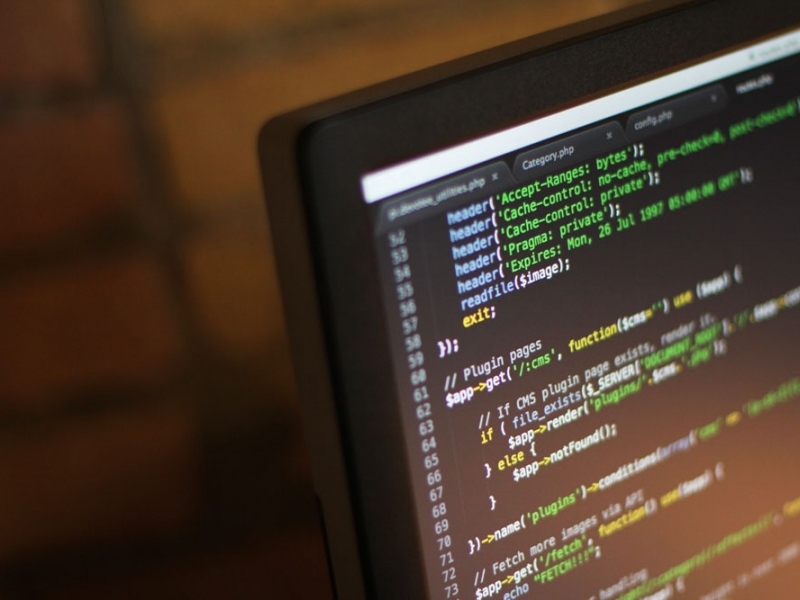
\includegraphics[width=0.7\textwidth,height=\textheight]{tex2pdf.-a0d3bc333fd33c29/ee62f68625d09ecdc466e7deaa763b4f88300352.jpg}
\caption{Название рисунка}\label{fig:001}
}
\end{figure}

\hypertarget{ux432ux44bux432ux43eux434ux44b}{%
\chapter{Выводы}\label{ux432ux44bux432ux43eux434ux44b}}

Здесь кратко описываются итоги проделанной работы.

\hypertarget{ux441ux43fux438ux441ux43eux43a-ux43bux438ux442ux435ux440ux430ux442ux443ux440ux44b}{%
\chapter*{Список
литературы}\label{ux441ux43fux438ux441ux43eux43a-ux43bux438ux442ux435ux440ux430ux442ux443ux440ux44b}}
\addcontentsline{toc}{chapter}{Список литературы}

\hypertarget{refs}{}
\begin{CSLReferences}{0}{0}
\leavevmode\vadjust pre{\hypertarget{ref-gnu-doc:bash}{}}%
\CSLLeftMargin{1. }
\CSLRightInline{{GNU Bash Manual} {[}Электронный ресурс{]}. Free
Software Foundation, 2016. URL:
\url{https://www.gnu.org/software/bash/manual/}.}

\leavevmode\vadjust pre{\hypertarget{ref-newham:2005:bash}{}}%
\CSLLeftMargin{2. }
\CSLRightInline{Newham C. {Learning the bash Shell: Unix Shell
Programming}. O’Reilly Media, 2005. 354 с.}

\leavevmode\vadjust pre{\hypertarget{ref-zarrelli:2017:bash}{}}%
\CSLLeftMargin{3. }
\CSLRightInline{Zarrelli G. {Mastering Bash}. Packt Publishing, 2017.
502 с.}

\leavevmode\vadjust pre{\hypertarget{ref-robbins:2013:bash}{}}%
\CSLLeftMargin{4. }
\CSLRightInline{Robbins A. {Bash Pocket Reference}. O’Reilly Media,
2016. 156 с.}

\leavevmode\vadjust pre{\hypertarget{ref-tannenbaum:arch-pc:ru}{}}%
\CSLLeftMargin{5. }
\CSLRightInline{Таненбаум Э. {Архитектура компьютера}. 6-е изд. СПб.:
Питер, 2013. 874 с.}

\leavevmode\vadjust pre{\hypertarget{ref-tannenbaum:modern-os:ru}{}}%
\CSLLeftMargin{6. }
\CSLRightInline{Таненбаум Э., Бос Х. {Современные операционные системы}.
4-е изд. СПб.: Питер, 2015. 1120 с.}

\end{CSLReferences}

\printbibliography

\end{document}
